\subsection{Purpose}

Task C evaluates the electronic structure of the relaxed magnetic ground-state
structures identified in Task B.  For Ni, the calculation uses the relaxed
ferromagnetic PBE structure.  For NiO, two AFM-II structures are analyzed: the
relaxed PBE structure and the relaxed DFT+\(U\) structure.  Keeping both NiO
cases is useful because the main physical question is not only whether NiO is
insulating, but also how the Hubbard correction changes the Ni \(3d\) and O
\(2p\) states near the band gap.

\subsection{Computational Setup and Assumptions}

Each electronic-structure case was split into three calculations:
\begin{itemize}
  \item \texttt{scf}: a self-consistent calculation on a regular
  Gamma-centered k-point mesh, writing \texttt{CHGCAR};
  \item \texttt{dos}: a fixed-charge calculation with \texttt{ICHARG = 11},
  a denser regular k-point mesh, \texttt{LORBIT = 11}, and
  \texttt{NEDOS = 3001};
  \item \texttt{bands}: a fixed-charge line-mode calculation with
  \texttt{ICHARG = 11} along a high-symmetry k-point path.
\end{itemize}

This is the standard VASP procedure for band structures and DOS: first obtain a
self-consistent charge density on a full Brillouin-zone mesh, then reuse that
charge density for non-self-consistent eigenvalues and DOS
\cite{vasp-band-structure,vasp-icharg}.  \texttt{ICHARG = 11} keeps the charge
density fixed and reads it from \texttt{CHGCAR}; VASP explicitly recommends
this mode for band-structure eigenvalues and DOS of a previously converged
charge density \cite{vasp-icharg}.  \texttt{LORBIT = 11} was used because it
prints site- and angular-momentum-resolved projections to \texttt{DOSCAR} and
\texttt{PROCAR}; these projections are qualitative PAW-projector weights, but
they are the standard VASP output for PDOS and projected bands
\cite{vasp-lorbit,vasp-doscar,vasp-procar}.

The SCF meshes were the conservative Task A/Task B production meshes:
\(24\times24\times24\) for Ni and \(16\times16\times16\) for NiO.  The DOS
meshes were increased to \(32\times32\times32\) for Ni and
\(20\times20\times20\) for NiO in order to sample the Fermi-level DOS and band
edges more smoothly.  Gamma-centered meshes were kept because the project had
already converged Gamma-centered meshes in Task A and because the VASP
\texttt{KPOINTS} documentation recommends symmetry-compatible regular meshes
for production calculations \cite{vasp-kpoints}.

\subsection{k-point Paths}

The band paths were chosen manually from standard high-symmetry-path
conventions.  The general convention follows Setyawan and Curtarolo's AFLOW
standardization of Bravais-lattice band paths \cite{setyawan-curtarolo}, and
the more recent crystallographic band-path framework of Hinuma \emph{et al.},
which is implemented in SeeK-path \cite{hinuma-seekpath}.  VASP's
\texttt{KPOINTS} documentation also recommends high-symmetry line-mode paths
for band-structure visualization and gives fcc high-symmetry coordinates as an
example \cite{vasp-kpoints}.  The line-mode calculations used 40 points per
line segment.

For fcc Ni, the path was
\[
  \Gamma - X - W - K - \Gamma - L - U - W - L.
\]
This is a standard fcc path containing the high-symmetry points commonly used
for fcc band structures; VASP also provides spin-polarized fcc Ni DOS and band
structure examples as a reference calculation \cite{vasp-fcc-ni}.  The current
VASP input uses the four-atom conventional cubic Ni cell, so the plotted bands
are folded with respect to a primitive fcc cell.  The labels are therefore best
understood as a conventional-cell representation of the fcc path rather than a
fully standardized primitive-cell SeeK-path output.

For NiO, the AFM-II cell is not the smallest cubic rocksalt cell.  It is a
two-Ni/two-O rhombohedral magnetic cell with alternating Ni moments along the
rocksalt \([111]\) direction.  Therefore the simple cubic rocksalt path was not
used.  Instead, a compact rhombohedral-style path was used:
\[
  \Gamma - L - B - \Gamma - Z - F - \Gamma.
\]
This path was chosen to sample inequivalent directions of the reciprocal cell
while keeping the calculation short enough for the present study.  A more
strict production calculation would generate the path directly from the relaxed
POSCAR using SeeK-path, but the present manually chosen path is sufficient for
the qualitative comparison required here.

\subsection{Results}

\begin{table}[h]
\centering
\caption{Task C electronic-structure summary.  The band gaps were extracted
from the dense uniform-mesh \texttt{dos/EIGENVAL} files, while the dominant
orbital characters were estimated from the PDOS within
\(\pm0.5~\mathrm{eV}\) of the Fermi level.}
\resizebox{\textwidth}{!}{%
\begin{tabular}{llllrl}
\toprule
System & Case & Character & Gap type & Gap (eV) & Dominant orbitals near \(E_F\) \\
\midrule
Ni  & PBE FM          & metallic   & metallic & 0.0002 & Ni \(d\), Ni \(p\), Ni \(s\) \\
NiO & PBE AFM-II      & insulating & indirect & 0.5970 & Ni \(d\), O \(p\), Ni \(p\) \\
NiO & DFT+\(U\) AFM-II & insulating & indirect & 3.4034 & O \(p\), Ni \(d\), Ni \(p\) \\
\bottomrule
\end{tabular}%
}
\end{table}

The tiny \(0.0002~\mathrm{eV}\) occupied/unoccupied separation reported for Ni
is only a numerical consequence of finite k-point sampling and should be
interpreted as zero gap.  The band structure and DOS show bands crossing the
Fermi level, as expected for metallic ferromagnetic Ni.  The DOS near
\(E_F\) is dominated by Ni \(3d\) character, with smaller Ni \(p\) and \(s\)
contributions.  This is consistent with Ni being a transition metal whose
partly filled \(d\)-derived bands control the low-energy electronic structure.

For PBE NiO, the AFM-II state is insulating, but the gap is only
\(0.597~\mathrm{eV}\).  This is much smaller than the historically measured
large gap of NiO, about \(4.3~\mathrm{eV}\) in the photoemission and inverse
photoemission study by Sawatzky and Allen \cite{sawatzky-allen-nio}.  The small
PBE gap is expected: semi-local DFT underestimates gaps and does not fully
describe the localized Ni \(3d\) correlation physics.  In the PBE result, the
states near the gap still have strong Ni \(d\) character mixed with O \(p\)
states, so the calculation captures antiferromagnetic insulating behavior but
not the experimental gap scale.

Adding the Hubbard correction opens the NiO gap to \(3.403~\mathrm{eV}\).  The
gap is still below the classic \(4.3~\mathrm{eV}\) experimental value, but it is
much closer than PBE and is in the expected range for a DFT+\(U\) description of
NiO.  The dominant character near the Fermi level changes from Ni \(d\)-first
in PBE to O \(p\)-first with important Ni \(d\) contribution in DFT+\(U\).  This
is physically meaningful: the Hubbard term pushes occupied and unoccupied Ni
\(d\) manifolds apart, increases \(d\)-state localization, and makes the gap
more charge-transfer-like.  This interpretation is consistent with the
Zaanen-Sawatzky-Allen picture, in which NiO is not a simple one-electron band
insulator but has mixed charge-transfer and Mott-Hubbard character
\cite{zaanen-sawatzky-allen,sawatzky-allen-nio}.

\begin{figure}[htbp]
\centering
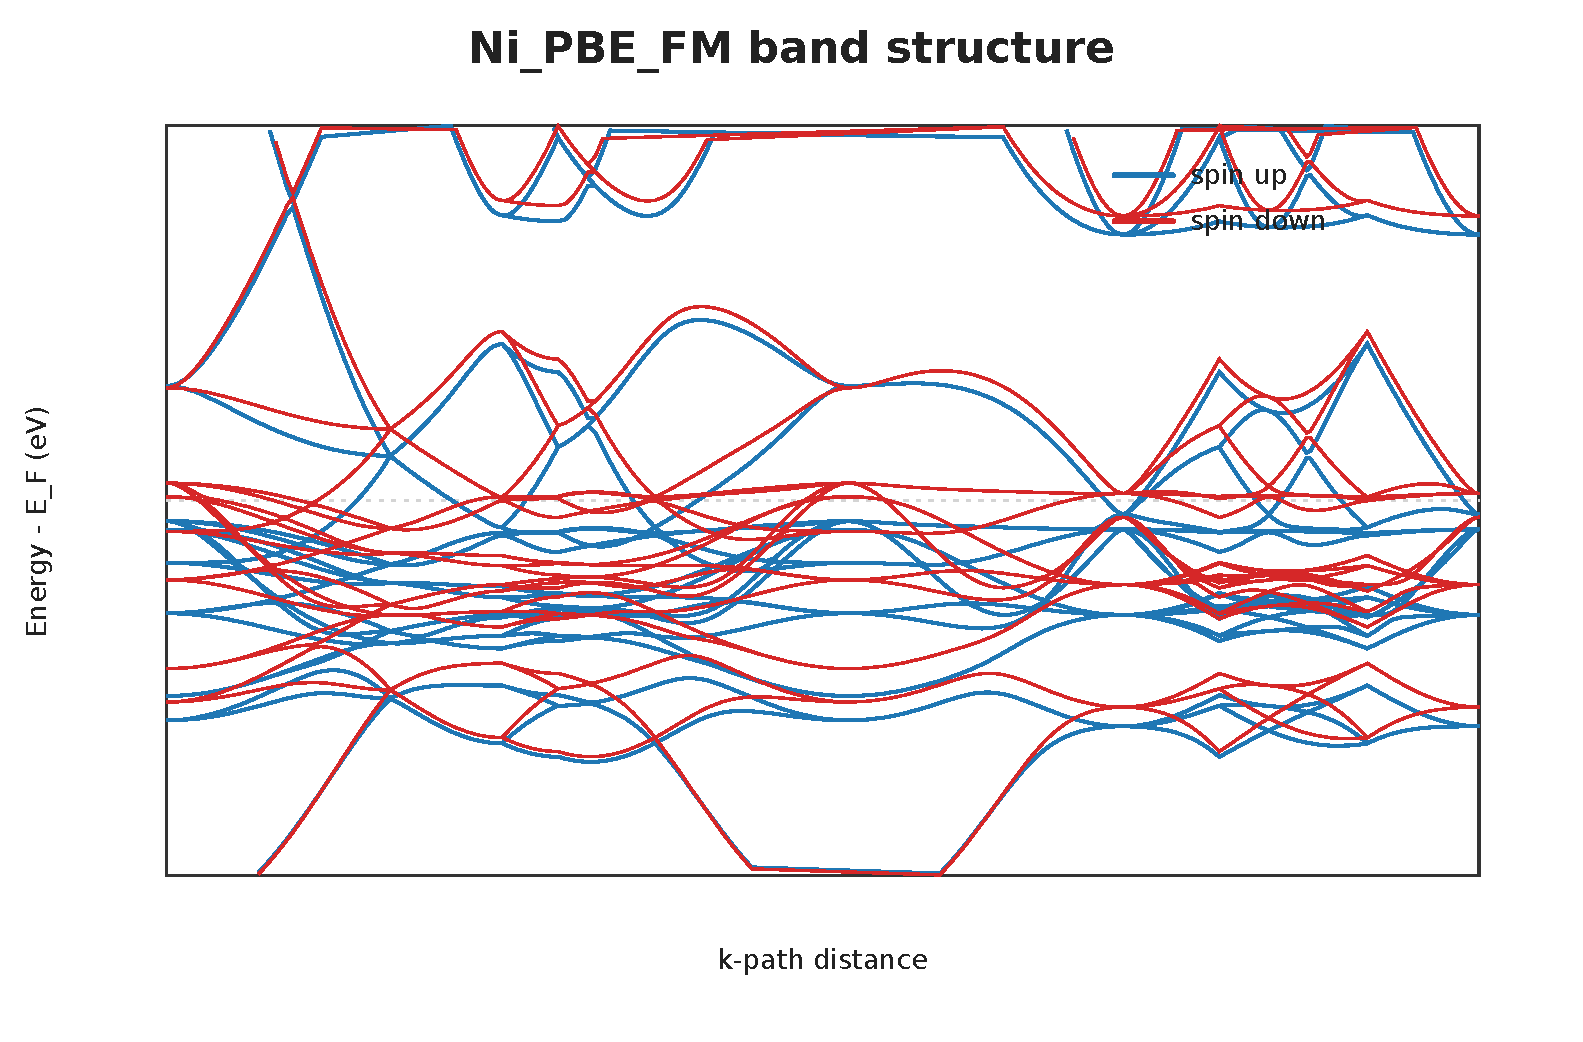
\includegraphics[width=\textwidth]{figures/Ni_PBE_FM_bands.pdf}
\caption{Band structure for ferromagnetic PBE Ni.  Energies are shifted so
that \(E_F = 0\).}
\label{fig:task-c-ni-bands}
\end{figure}

\begin{figure}[htbp]
\centering
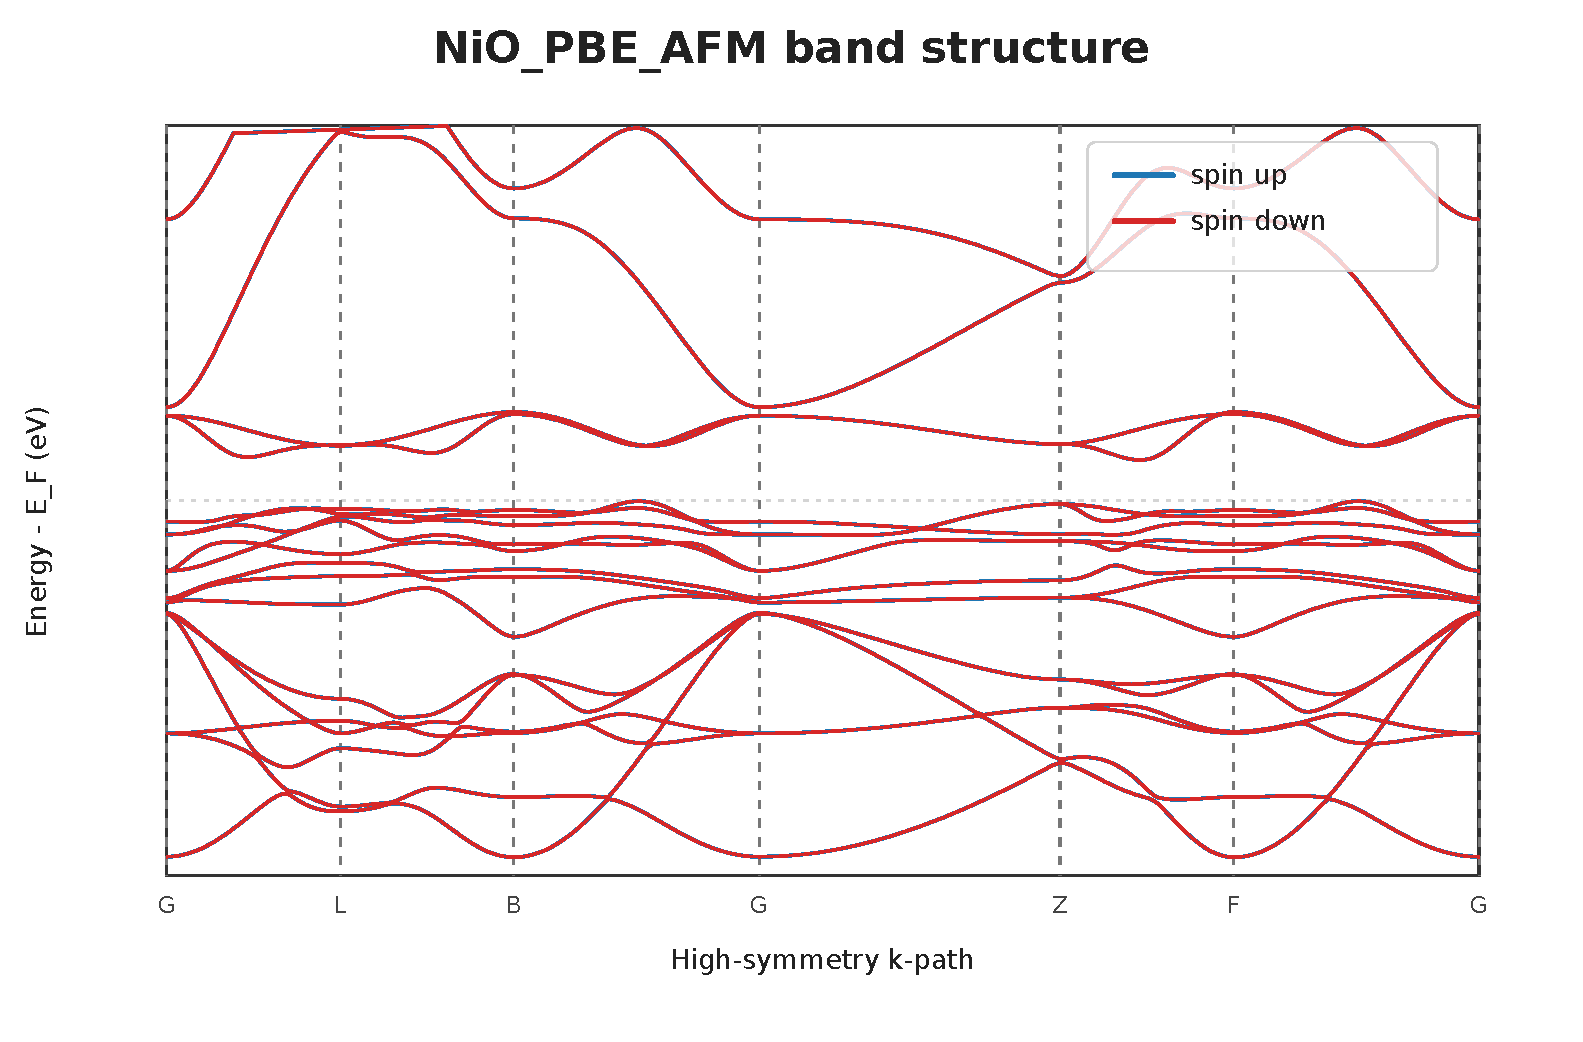
\includegraphics[width=\textwidth]{figures/NiO_PBE_AFM_bands.pdf}
\caption{Band structure for PBE NiO in the AFM-II ordering.  Energies are
shifted so that \(E_F = 0\).}
\label{fig:task-c-nio-pbe-bands}
\end{figure}

\begin{figure}[htbp]
\centering
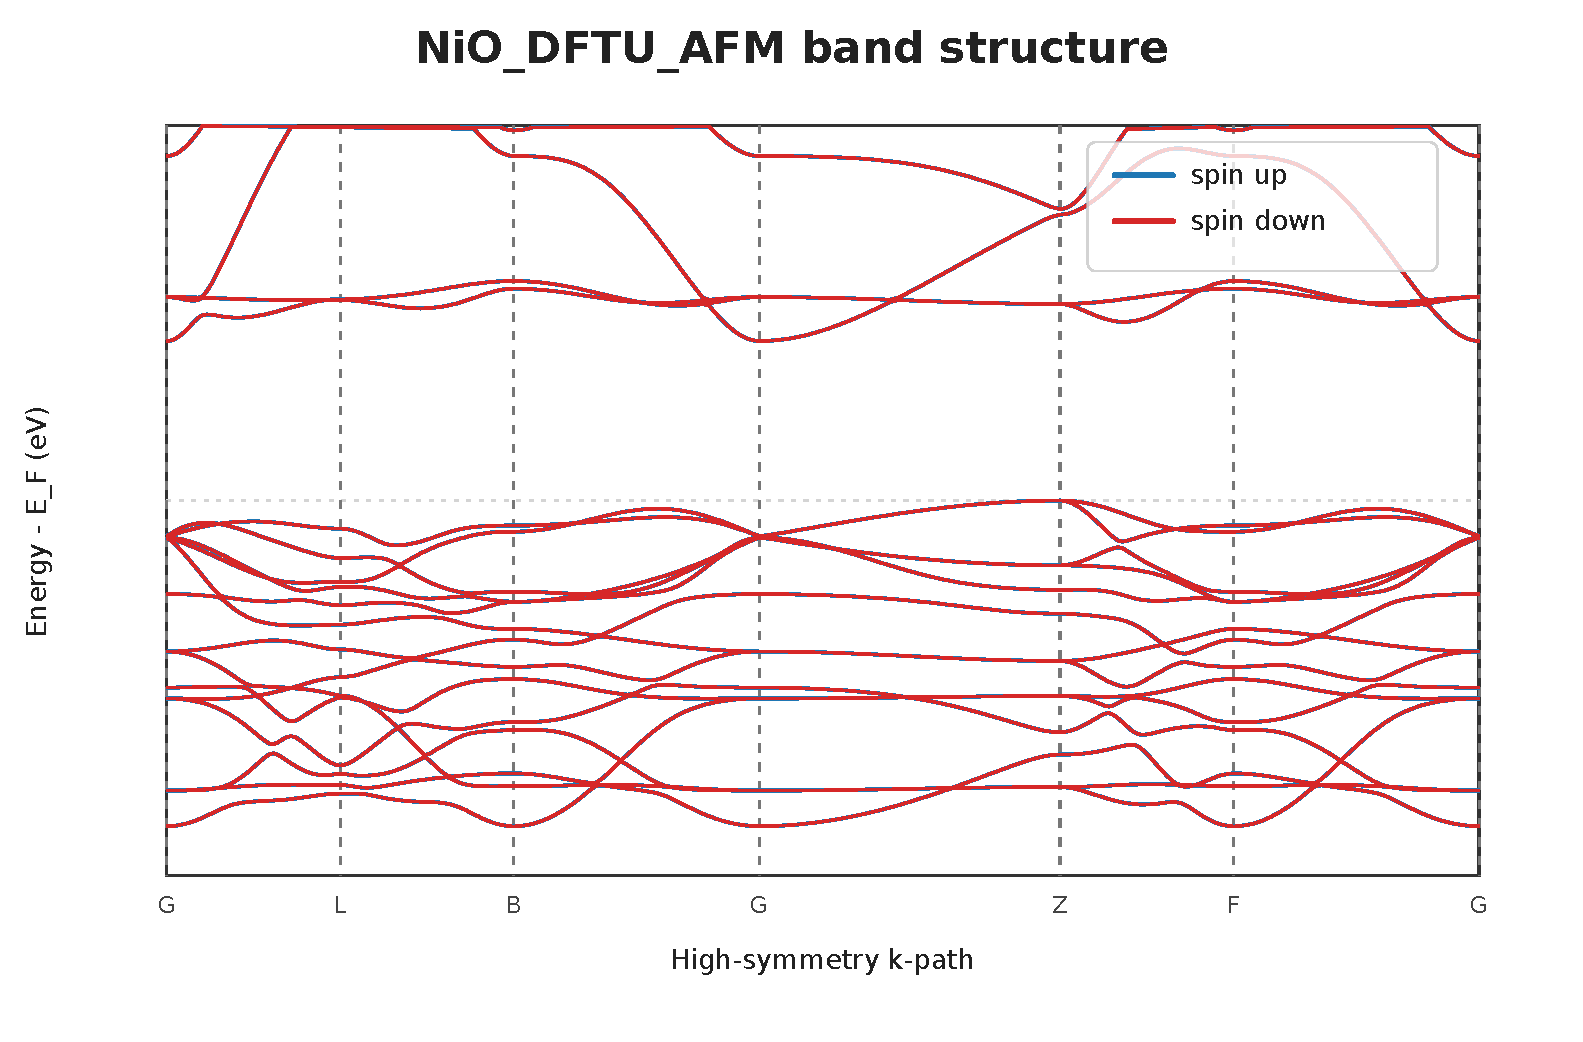
\includegraphics[width=\textwidth]{figures/NiO_DFTU_AFM_bands.pdf}
\caption{Band structure for DFT+\(U\) NiO in the AFM-II ordering.  Energies are
shifted so that \(E_F = 0\).}
\label{fig:task-c-nio-dftu-bands}
\end{figure}

\begin{figure}[htbp]
\centering
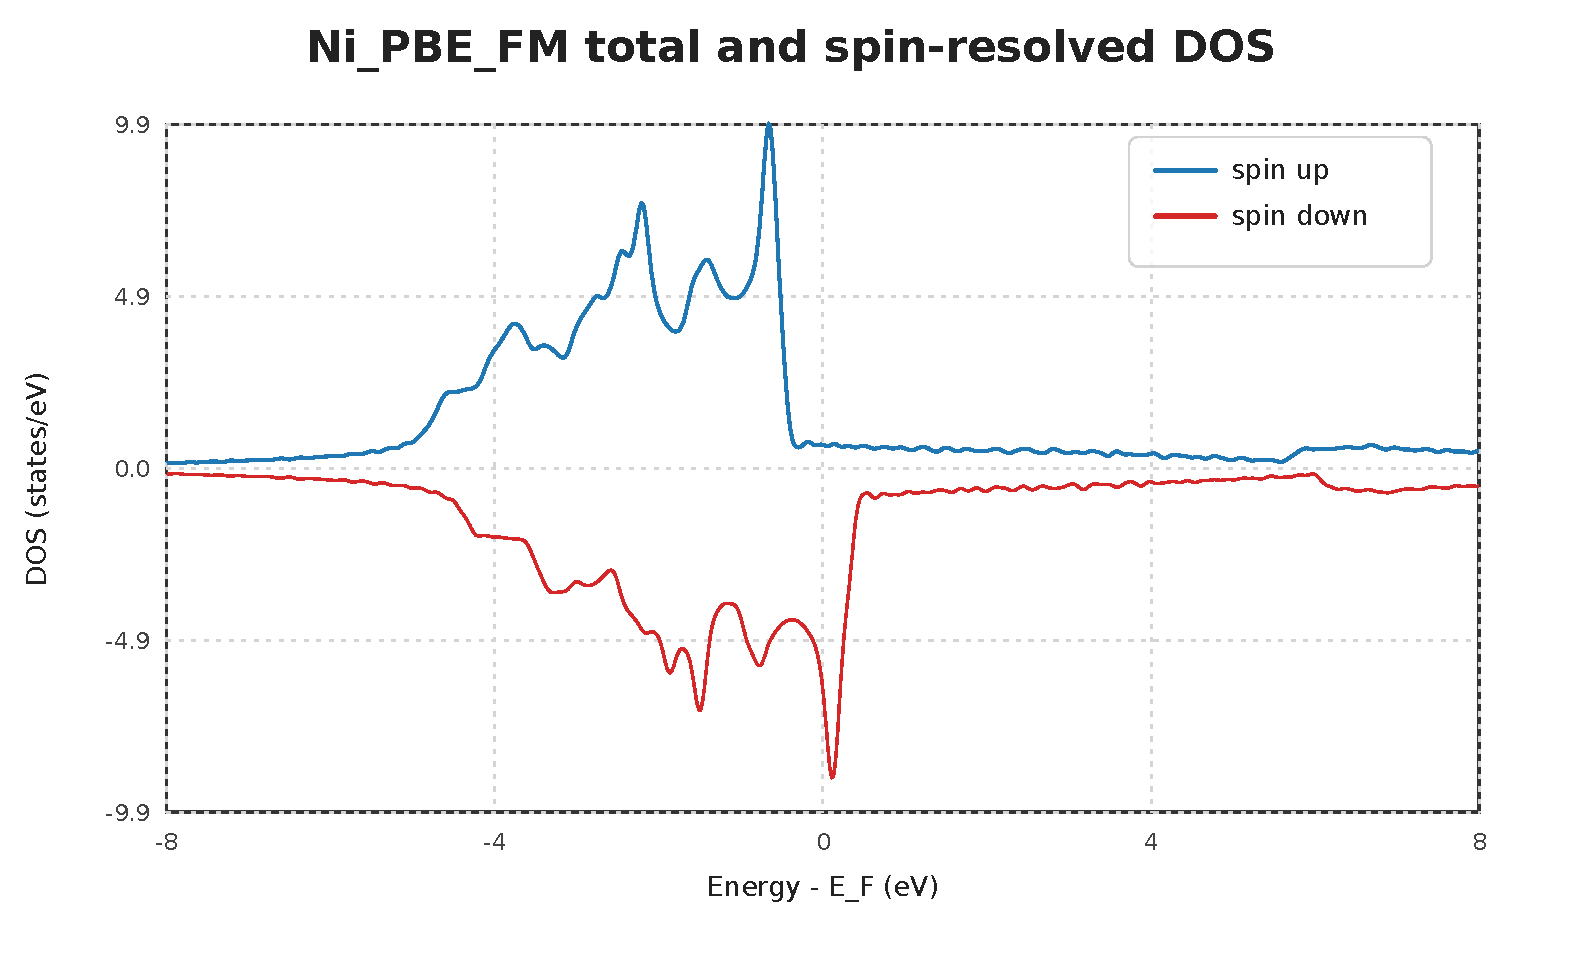
\includegraphics[width=\textwidth]{figures/Ni_PBE_FM_dos.pdf}
\caption{Total and spin-resolved DOS for ferromagnetic PBE Ni, showing finite
DOS at the Fermi level.}
\label{fig:task-c-ni-dos}
\end{figure}

\begin{figure}[htbp]
\centering
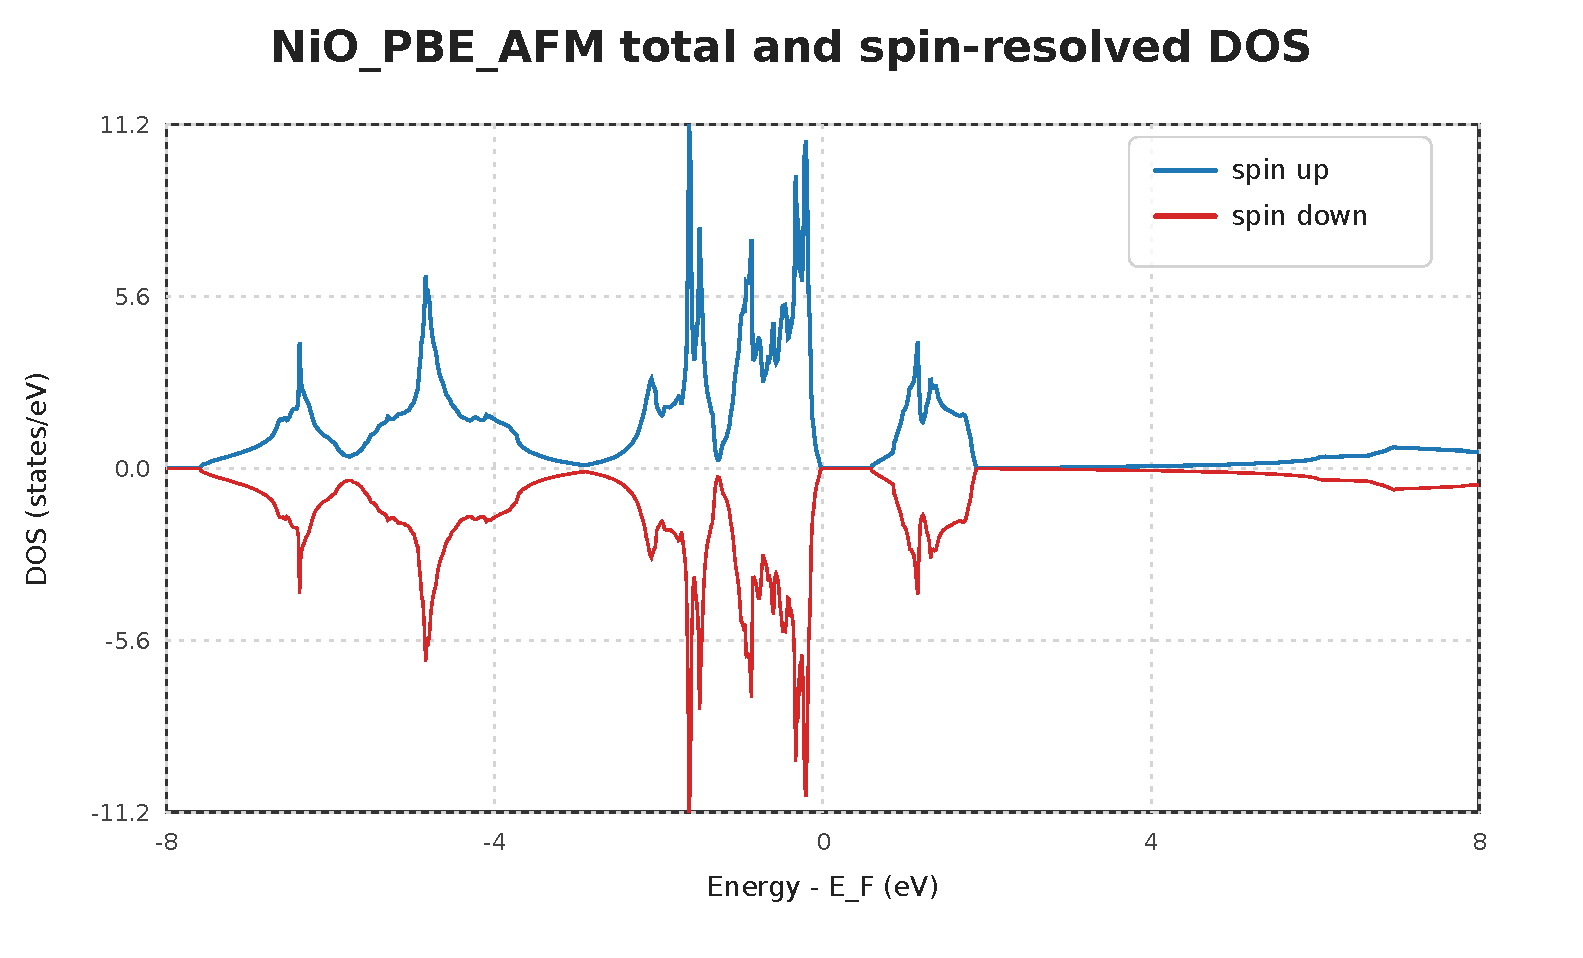
\includegraphics[width=\textwidth]{figures/NiO_PBE_AFM_dos.pdf}
\caption{Total and spin-resolved DOS for PBE NiO in the AFM-II ordering,
showing an insulating gap.}
\label{fig:task-c-nio-pbe-dos}
\end{figure}

\begin{figure}[htbp]
\centering
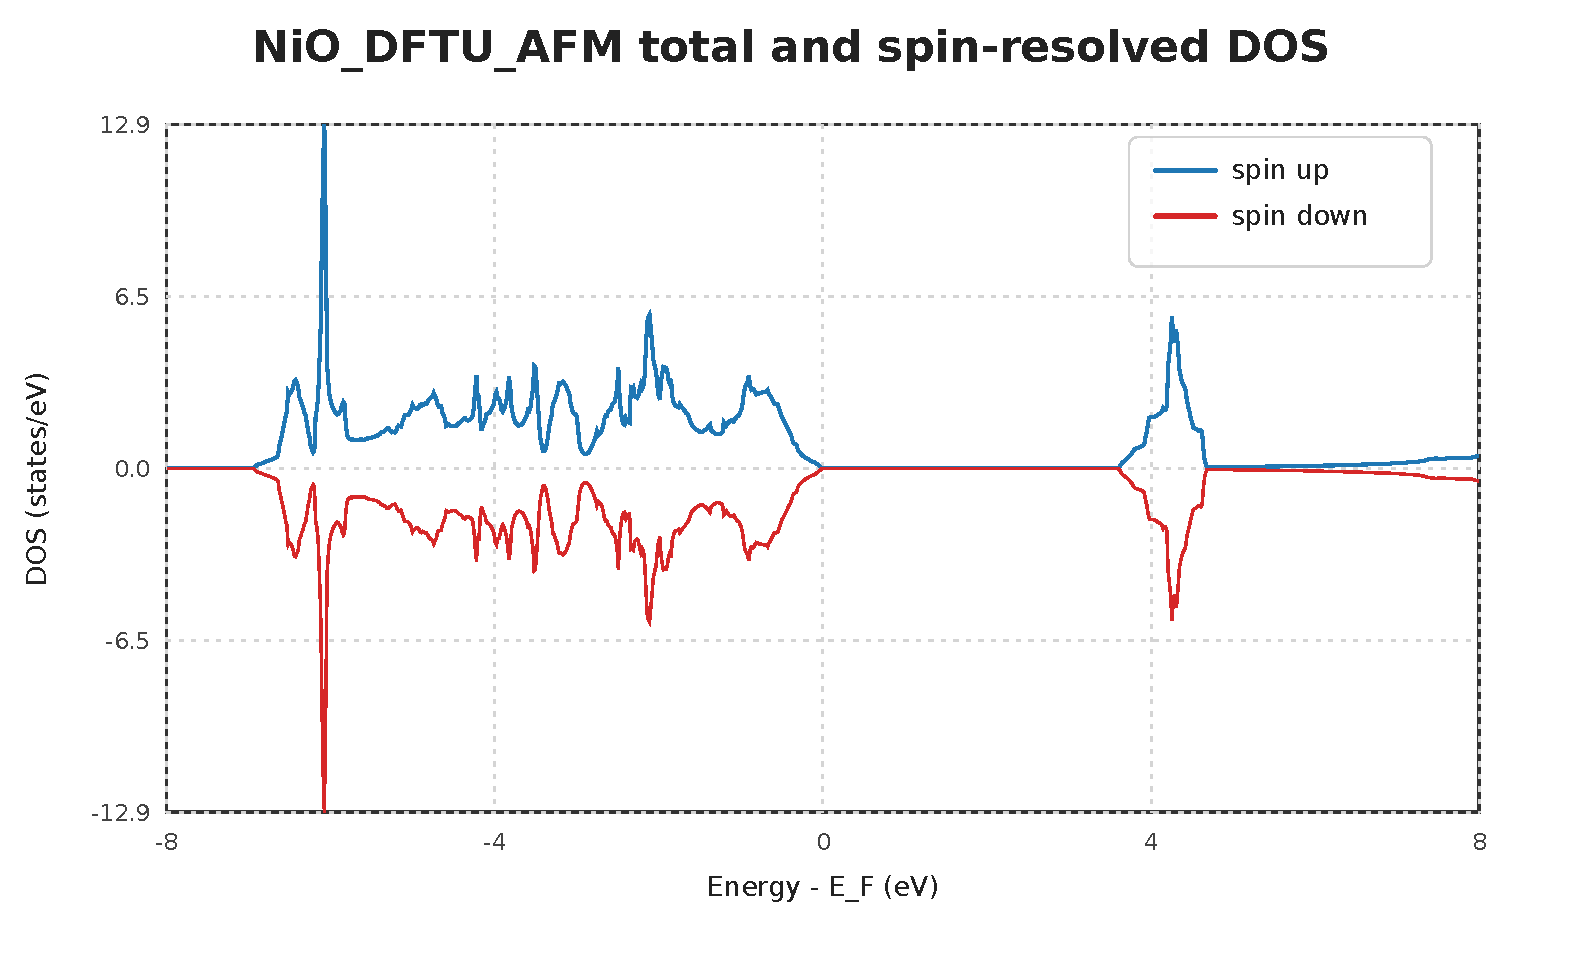
\includegraphics[width=\textwidth]{figures/NiO_DFTU_AFM_dos.pdf}
\caption{Total and spin-resolved DOS for DFT+\(U\) NiO in the AFM-II ordering,
showing the larger gap opened by the Hubbard correction.}
\label{fig:task-c-nio-dftu-dos}
\end{figure}

\begin{figure}[htbp]
\centering
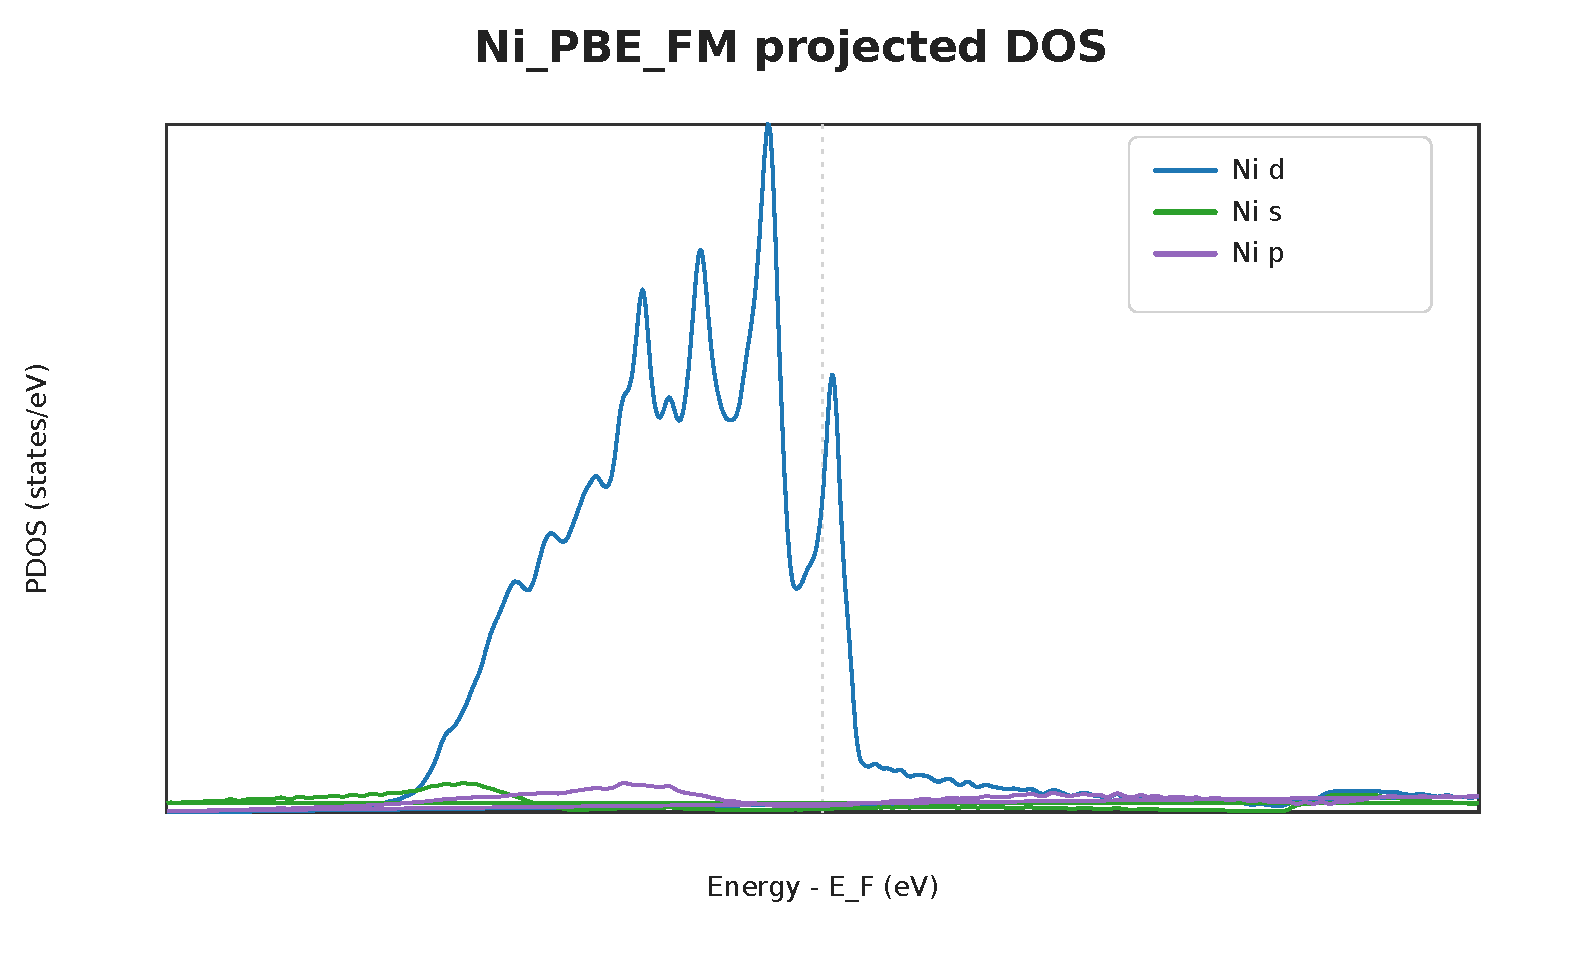
\includegraphics[width=\textwidth]{figures/Ni_PBE_FM_pdos.pdf}
\caption{Projected density of states for ferromagnetic PBE Ni.  The metal is
dominated by Ni \(d\)-derived states near \(E_F\).}
\label{fig:task-c-ni-pdos}
\end{figure}

\begin{figure}[htbp]
\centering
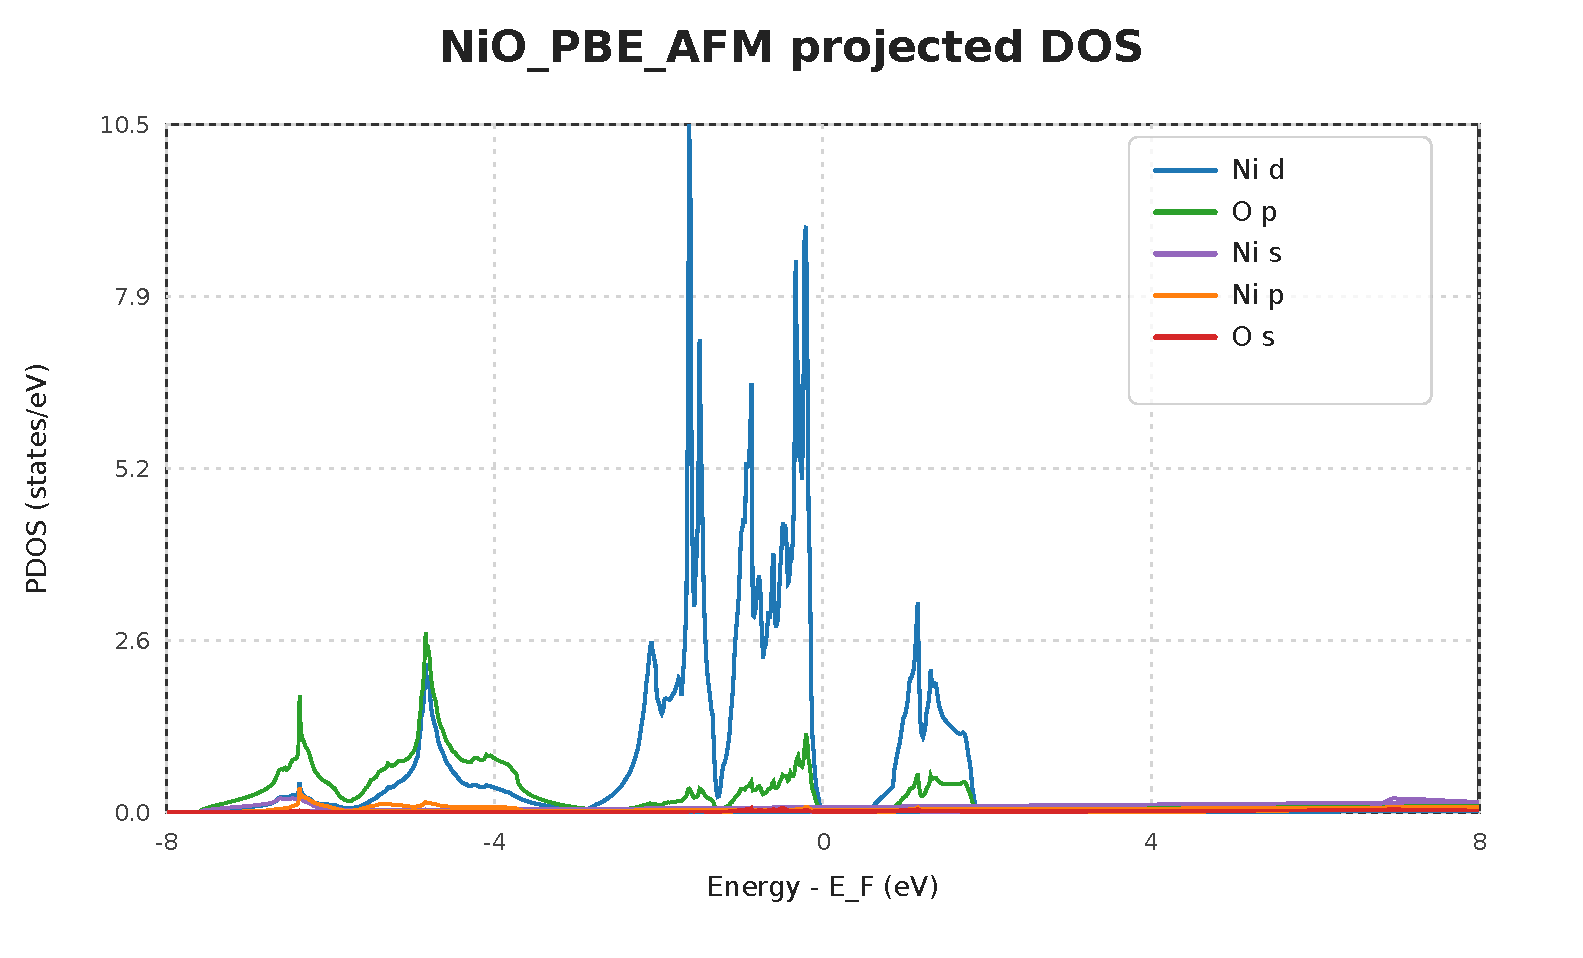
\includegraphics[width=\textwidth]{figures/NiO_PBE_AFM_pdos.pdf}
\caption{Projected density of states for PBE NiO in the AFM-II ordering.  O
\(p\) and Ni \(d\) states form the valence and conduction edges.}
\label{fig:task-c-nio-pbe-pdos}
\end{figure}

\begin{figure}[htbp]
\centering
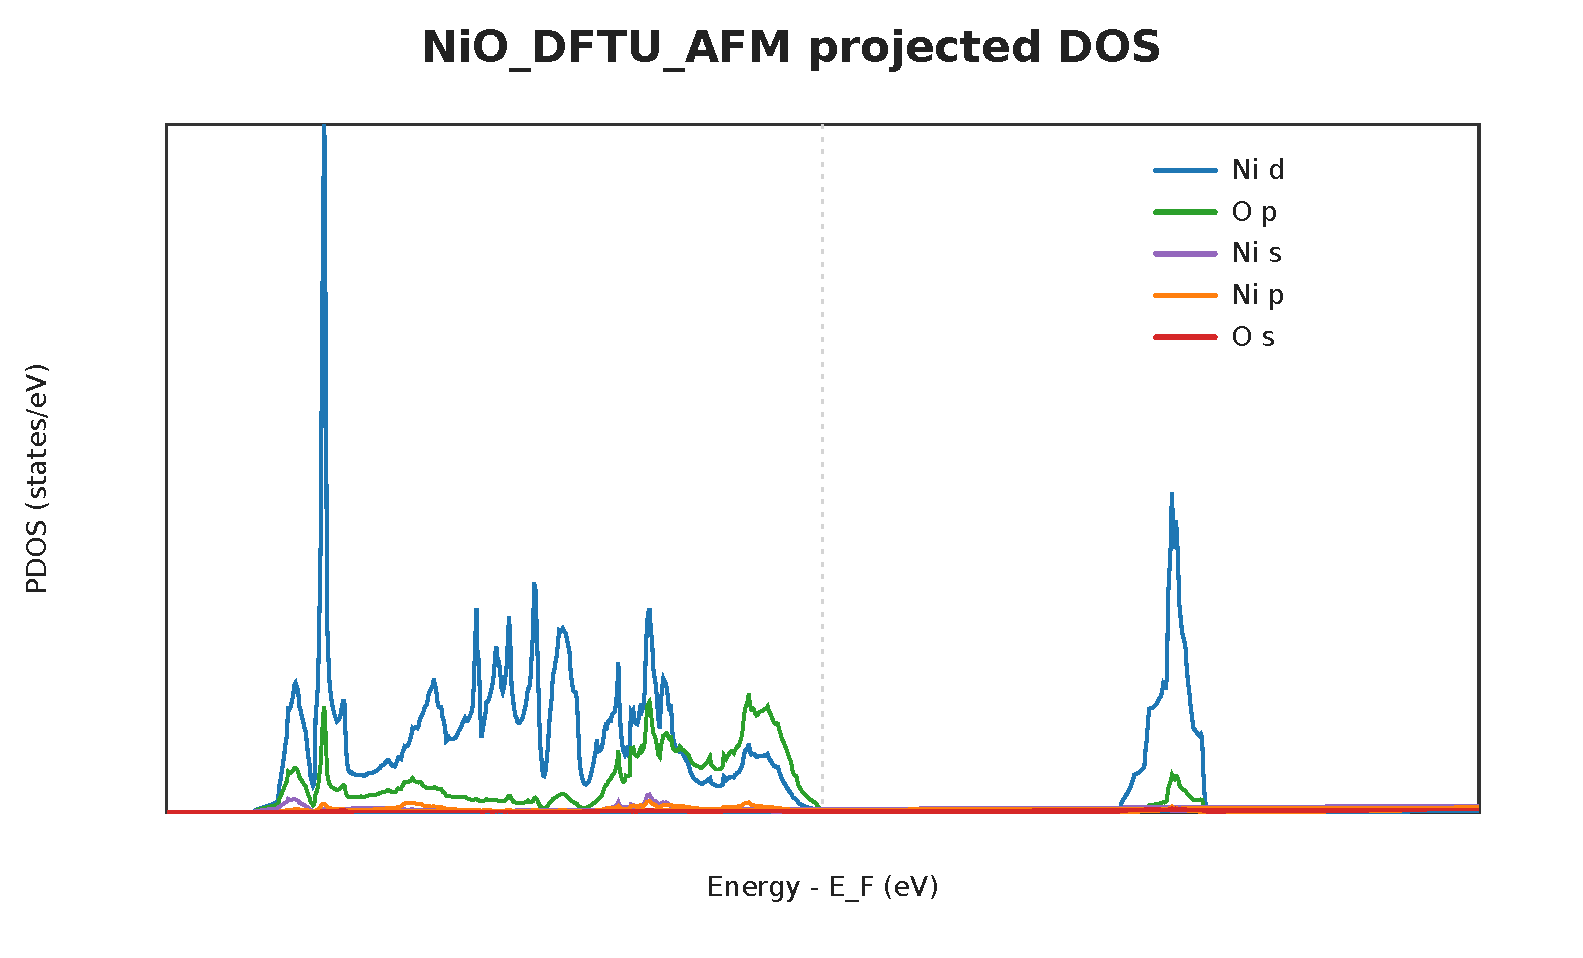
\includegraphics[width=\textwidth]{figures/NiO_DFTU_AFM_pdos.pdf}
\caption{Projected density of states for DFT+\(U\) NiO in the AFM-II ordering.
The Hubbard correction increases the separation between occupied and
unoccupied states.}
\label{fig:task-c-nio-dftu-pdos}
\end{figure}

\begin{figure}[htbp]
\centering
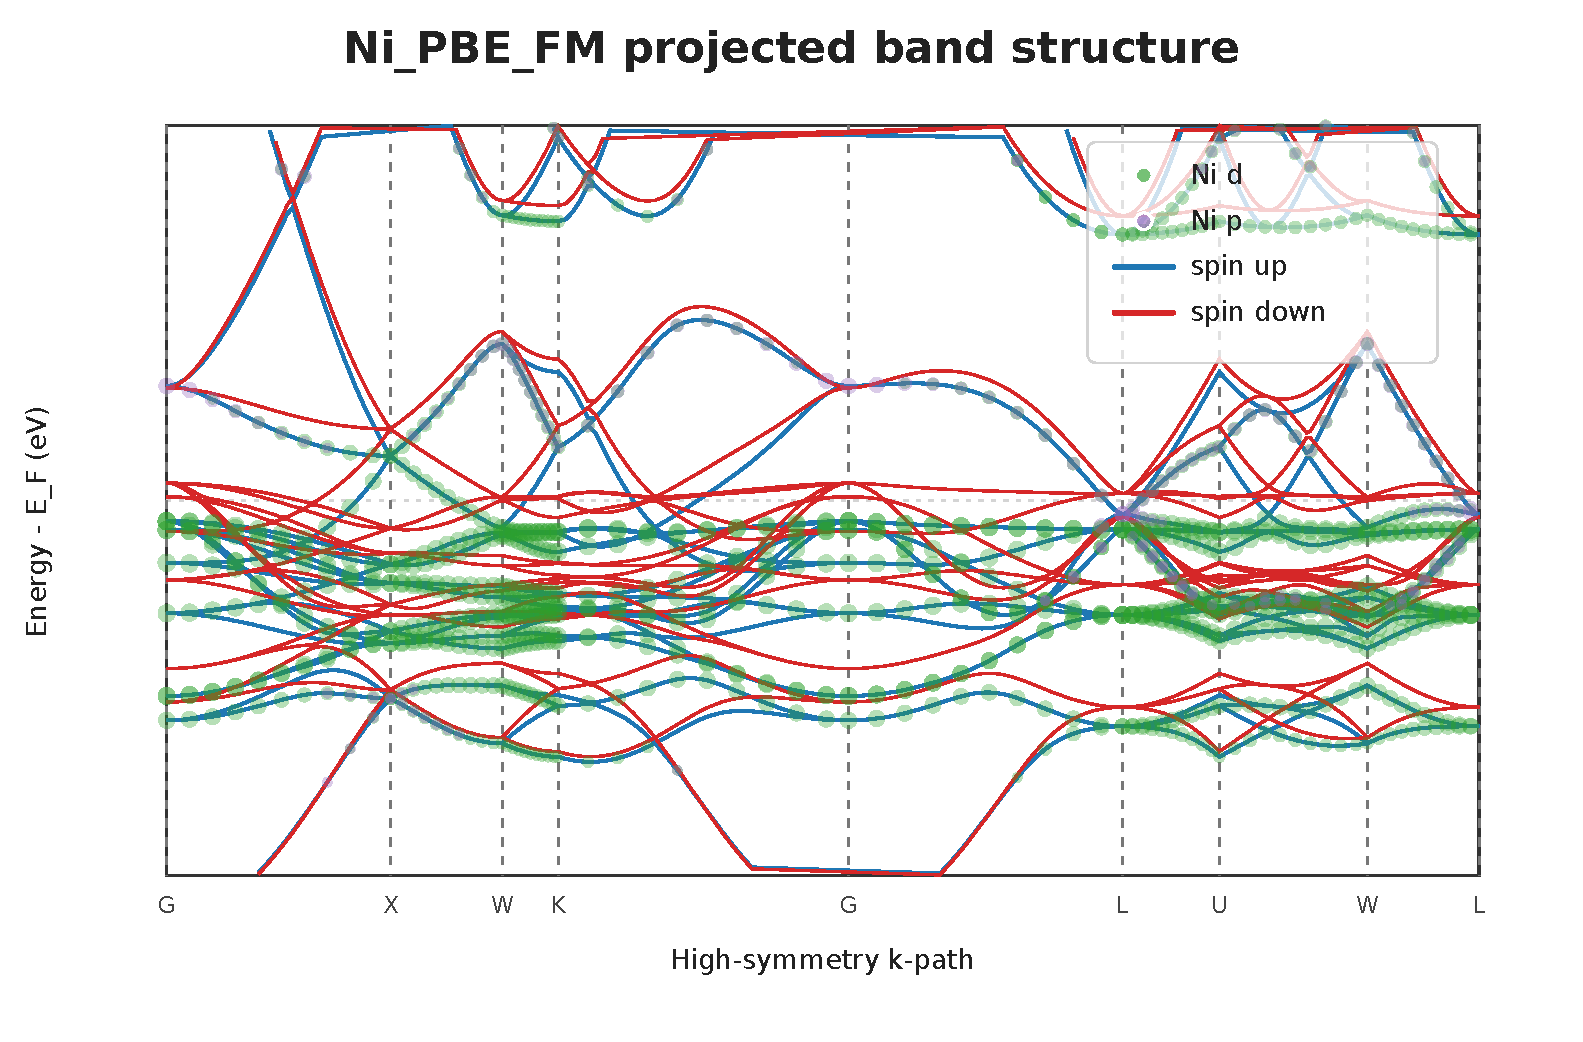
\includegraphics[width=\textwidth]{figures/Ni_PBE_FM_projected_bands.pdf}
\caption{Projected band structure for ferromagnetic PBE Ni.  Marker sizes are
proportional to selected \texttt{PROCAR} orbital weights, here Ni \(d\) and
Ni \(p\).}
\label{fig:task-c-ni-projected-bands}
\end{figure}

\begin{figure}[htbp]
\centering
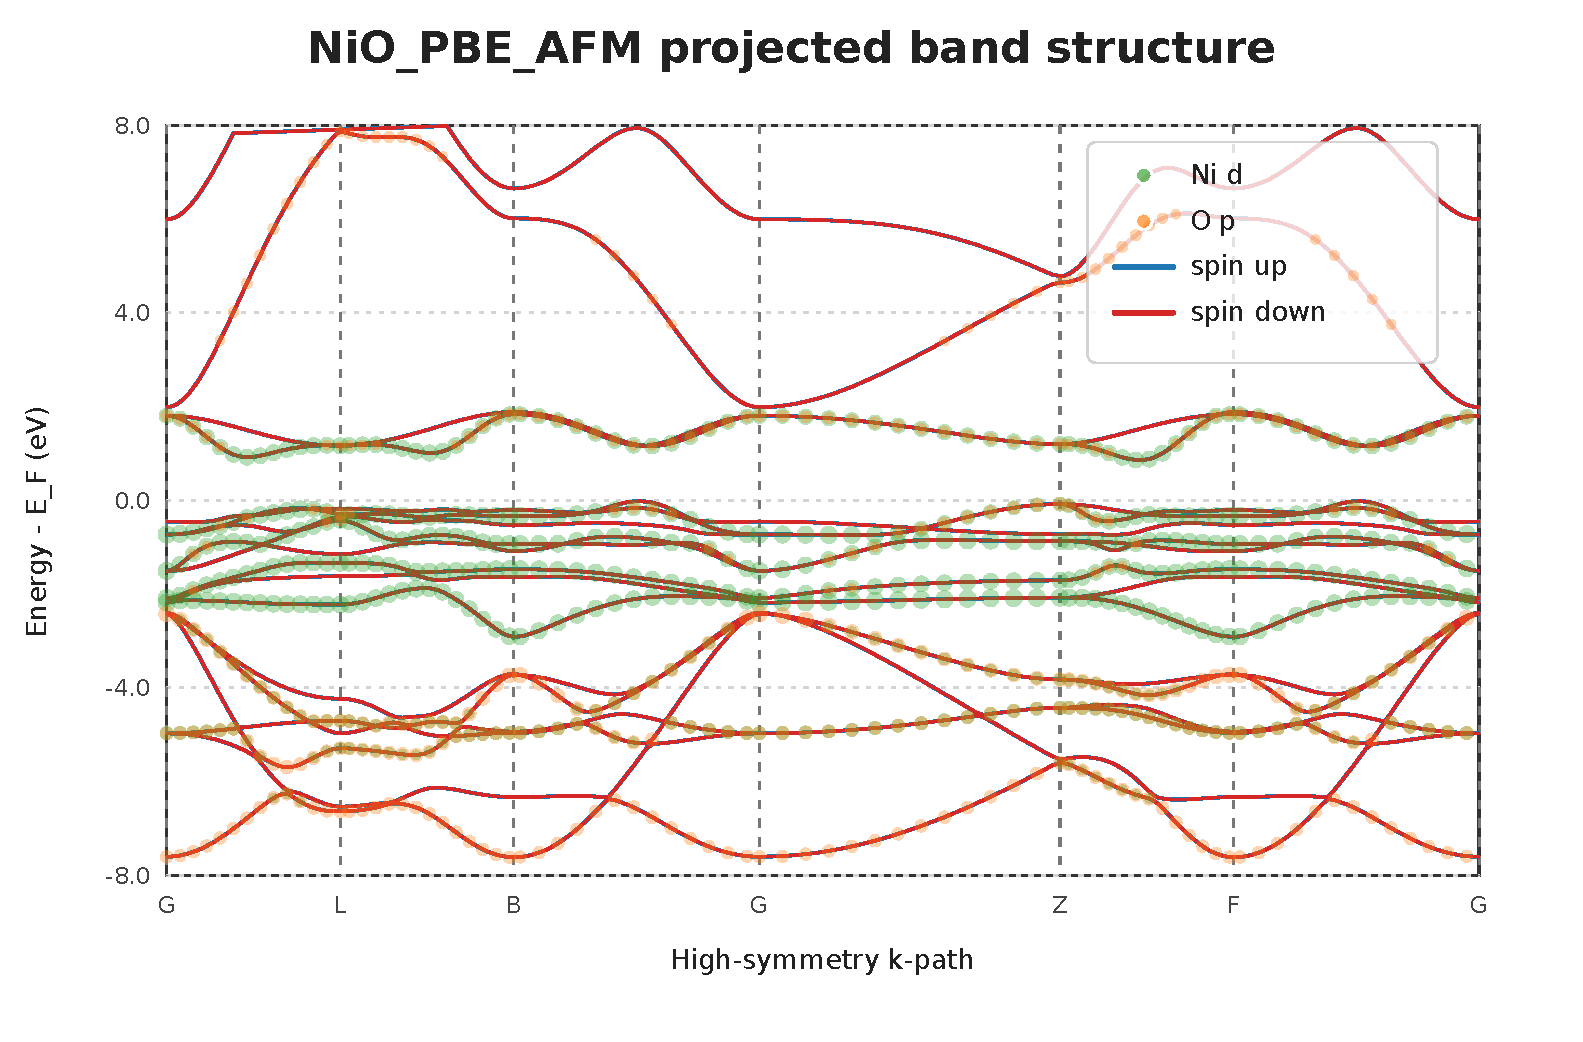
\includegraphics[width=\textwidth]{figures/NiO_PBE_AFM_projected_bands.pdf}
\caption{Projected band structure for PBE NiO in the AFM-II ordering.  Marker
sizes are proportional to selected \texttt{PROCAR} orbital weights, here
Ni \(d\) and O \(p\).}
\label{fig:task-c-nio-pbe-projected-bands}
\end{figure}

\begin{figure}[htbp]
\centering
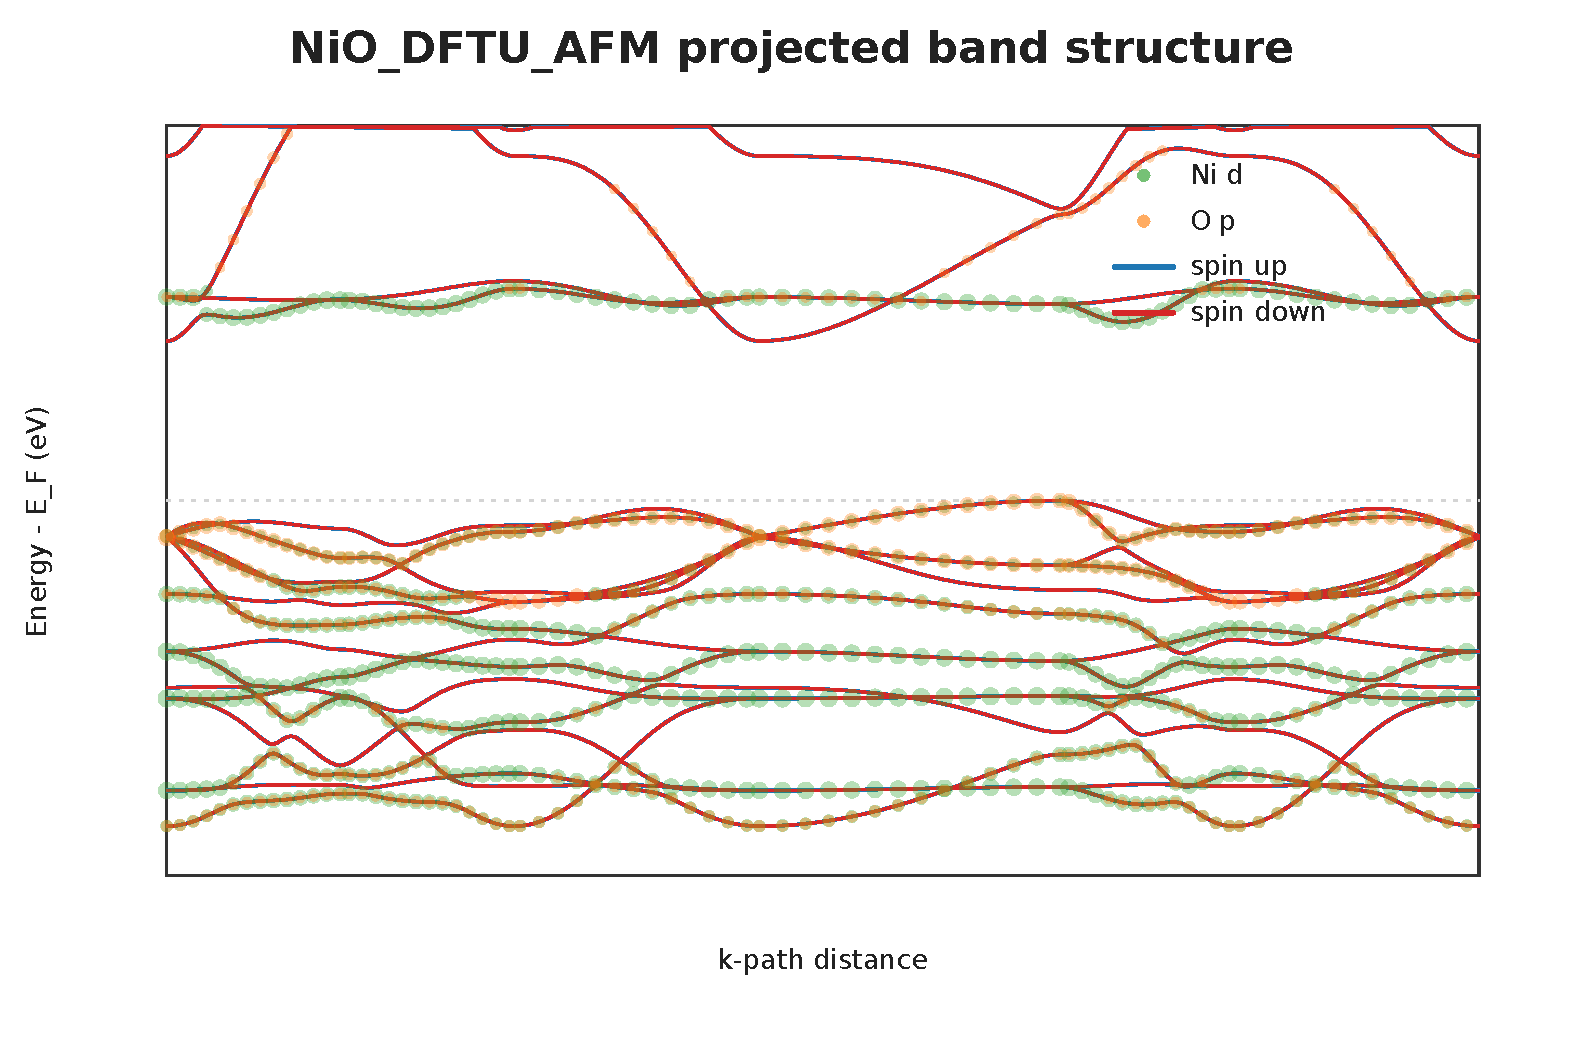
\includegraphics[width=\textwidth]{figures/NiO_DFTU_AFM_projected_bands.pdf}
\caption{Projected band structure for DFT+\(U\) NiO in the AFM-II ordering.
Marker sizes are proportional to selected \texttt{PROCAR} orbital weights,
here Ni \(d\) and O \(p\).}
\label{fig:task-c-nio-dftu-projected-bands}
\end{figure}

\subsection{Discussion}

The comparison between Ni and NiO shows the qualitative electronic change
caused by oxidation.  Metallic Ni has no gap and has Ni \(d\)-dominated states
at the Fermi level.  NiO, in contrast, becomes insulating once AFM-II magnetic
order is included, even at the PBE level.  However, PBE leaves the gap far too
small.  The DFT+\(U\) correction opens the gap substantially and moves the
result toward the experimentally observed large-gap insulating behavior of NiO.

The projected DOS and projected band plots should be read as qualitative
orbital-character indicators rather than as unique decompositions of the
electronic states.  The PAW projection weights depend on the projector spheres
and on the chosen local-orbital channels, but they are still useful for the
main comparison made here: PBE leaves substantial Ni \(d\) weight at the band
edges, whereas DFT+\(U\) pushes the occupied and unoccupied Ni \(d\) manifolds
apart and makes the valence edge more oxygen-\(p\)-like.  This is exactly the
trend expected for a correlated charge-transfer oxide.

The manually chosen NiO band path is sufficient for comparing PBE and DFT+\(U\)
on the same relaxed magnetic cell, but it should not be interpreted as a fully
standardized primitive-cell band path.  Consequently, the robust conclusions of
Task C are the metallic versus insulating character, the size and trend of the
gap, and the change in orbital character; detailed assignment of every band
extremum would require a symmetry-standardized path generated directly from the
relaxed magnetic structure.

The total magnetic moment in the AFM-II NiO calculations is zero because the
two Ni sublattice moments cancel, not because the Ni atoms are non-magnetic.
This is consistent with Task B, where the local Ni moments were finite and
opposite in sign.  The electronic-structure results therefore support the same
physical picture as the structural and magnetic calculations: elemental Ni is a
ferromagnetic metal, while NiO is an antiferromagnetic correlated insulator
whose low-energy electronic structure is controlled by hybridized O \(2p\) and
Ni \(3d\) states.
